%\section{A closer look at the quality issues}
\section{Design Space}
To meet the delay constraints, there are two kinds of solution. One is to limit the size of the sender buffer, strictly restrain each frame to meet the requirements; the other maybe controlled by scheduling to maintain the average of delay at the target value. In our case, the first one is our choice. We limit the buffer size to $0.9s$. 

With buffer size limited, the previous case study gives us three intuitions to improve the video streaming quality.
\subsection{Design Space Insight}
\textbf{Eliminate the dependency between frames.}
By this means, the solution space would be larger and more optimal solutions are expected to be found.

There are two ways to implement this constraint relaxation. A naive approach is to reduce the keyframe interval. For example, if a 2-second interruption starts at the beginning of an 8-second GOP, the whole group are dropped; but if the 8-second GOP is refined to be four 2-second GOP, only one 2-second GOP would be dropped. Thus, the cascading effect would be eliminated. However, this approach may be a tradeoff between the minimal frame drop and the video quality, because reducing keyframe interval means less compression in video streaming, to keep a pre-configured bitrate, per-image quality would be degraded (i.e., ``big pixels''). The method needs a good tradeoff between video quality and frame dropping.

Another approach is to make the GOP selection adapt to the network condition. In details, when the network recovers from an interruption, the first frame transmitted is encoded as I frame, and a new GOP restarts from this first frame. In this way, the new GOP has no dependency with previous (possible dropped) frames, and all its frames are decodable. This approach may need to modify the encoding workflow, which is hard and out of control.

%\textbf{Relax queue length threshold.} In the model, if we make $T_1$ larger, the applicable solution space is also larger. The tradeoff of this method is that frames during the interruption are accumulated at the queue, and whenever the network recovers, the ``stale'' frames in the queue would be transmitted first, causing display delay (not real-time) on the audience side.

\textbf{Improve the frame drop strategy.} Compared with the naive strategy in OBS (dropping all P/B in buffer when exceeding a threshold), intuitively, dropping frames within the old GoP, rather than all, may have better performance. It is worth thinking how to design an online frame dropping strategy that approaches the optimal solution. The challenge is the complexity of the frame management mechanism. A brute force solution is impossible because its time complexity.

\textbf{Adaptive bitrate.} Network condition is always changing along time. Conclusions from figure~\ref{fig:trace-all} validate the fact. Previous broadcasters can only use constant bitrate, CBR or ABR, which means the actual bitrate varies among the target value, at most down or up $20\%$ of the target bitrate. These two methods cannot follow the changing bandwidth, which would bring tremendous frame dropping when bandwidth falls down. Especially in the case where the bandwidth drop lasts for a long while. One possible solution is like DASH in VOD scenario, we use adaptive bitrate in broadcaster's side. Introducing bitrate adaptation maybe dramatically cut down the frame dropping.

\iffalse
\begin{itemize}
\item If we can relax the dependency between frames, the solution space would be larger and more optimal solutions are expected to be found. That is, we can relax the decodability constraints to be $d_i = 1, \forall i$.

\item We can relax queue length constraint, i.e., making $T_1$ larger. This change similarly increases the space of possible solutions.

\item The frame drop strategy can be improved. That is, compared with the naive strategy in OBS (dropping all P/B when exceeding a threshold), selectively choosing frames to drop in IP would give a more optimal solution.
\end{itemize}
\fi

\subsection{Preliminary Evaluation}
\textbf{Implementation and experiment setup.} In this section, we evaluate two methods: reducing keyframe interval, and changing the bitrate. We design control experiments, where we control the bitrate to a certain level, and introduces a 2-second interruption. We record the number of frame drop as metrics to evaluate these methods.

\begin{figure}[htb]
\centering
\begin{subfigure}[b]{.8\columnwidth}
\centering
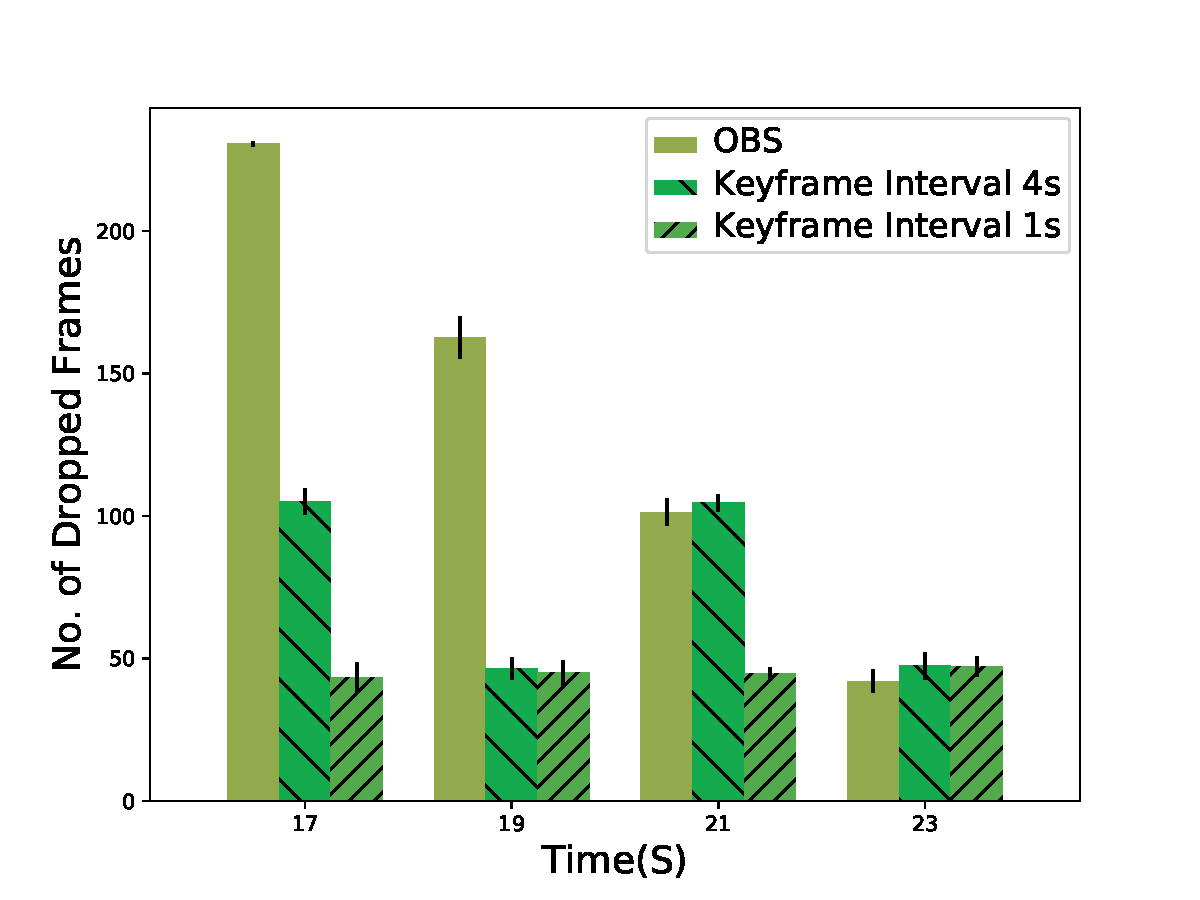
\includegraphics[width=\textwidth]{fig/eval_IframeInterval_drop.pdf}
\caption{Frame drop with varying I frame interval}
\label{fig:iframe-drop}\mylabel{fig:iframe-drop}
\end{subfigure}

\iffalse
\minipage{0.32\textwidth}
  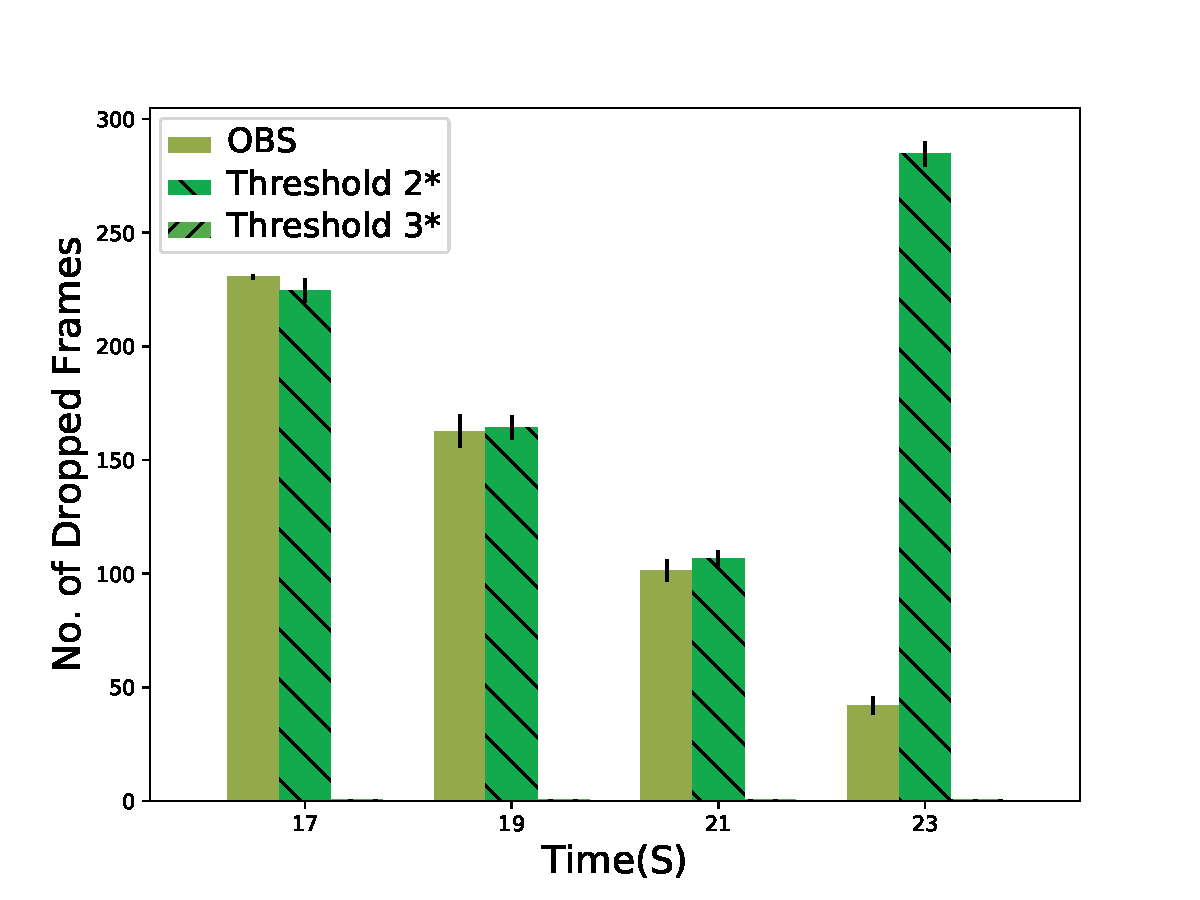
\includegraphics[width=\linewidth]{fig/eval_threshold_drop.pdf}
  \caption{Frame drop with varying threshold}
  \label{fig:threshold-drop}\mylabel{fig:threshold-drop}
\endminipage\hfill
\minipage{0.32\textwidth}
  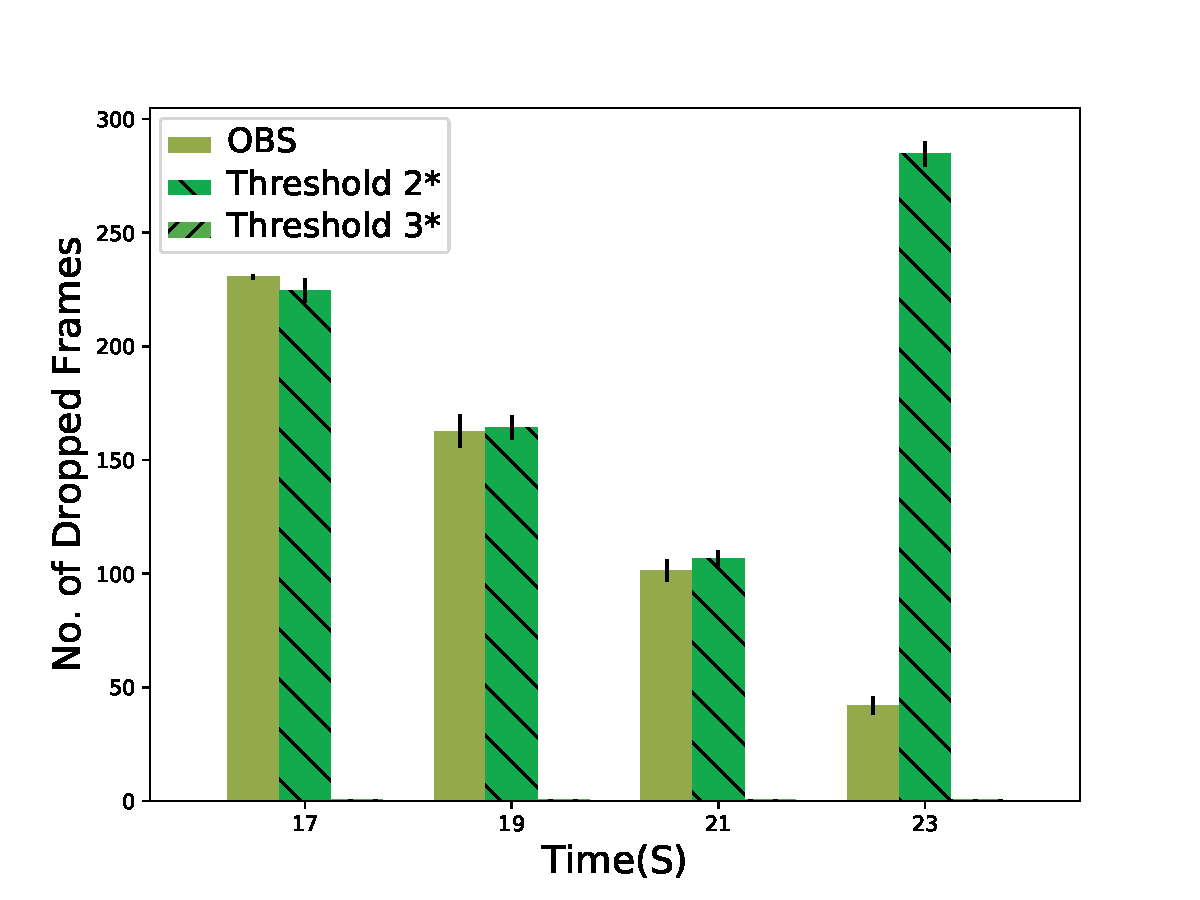
\includegraphics[width=\linewidth]{fig/eval_threshold_drop.pdf}
  \caption{Timeliness with varying I frame interval}
  \label{fig:iframe-timeliness}\mylabel{fig:iframe-timeliness}
\endminipage
\fi

\end{figure}

\iffalse
\begin{figure}
\centering
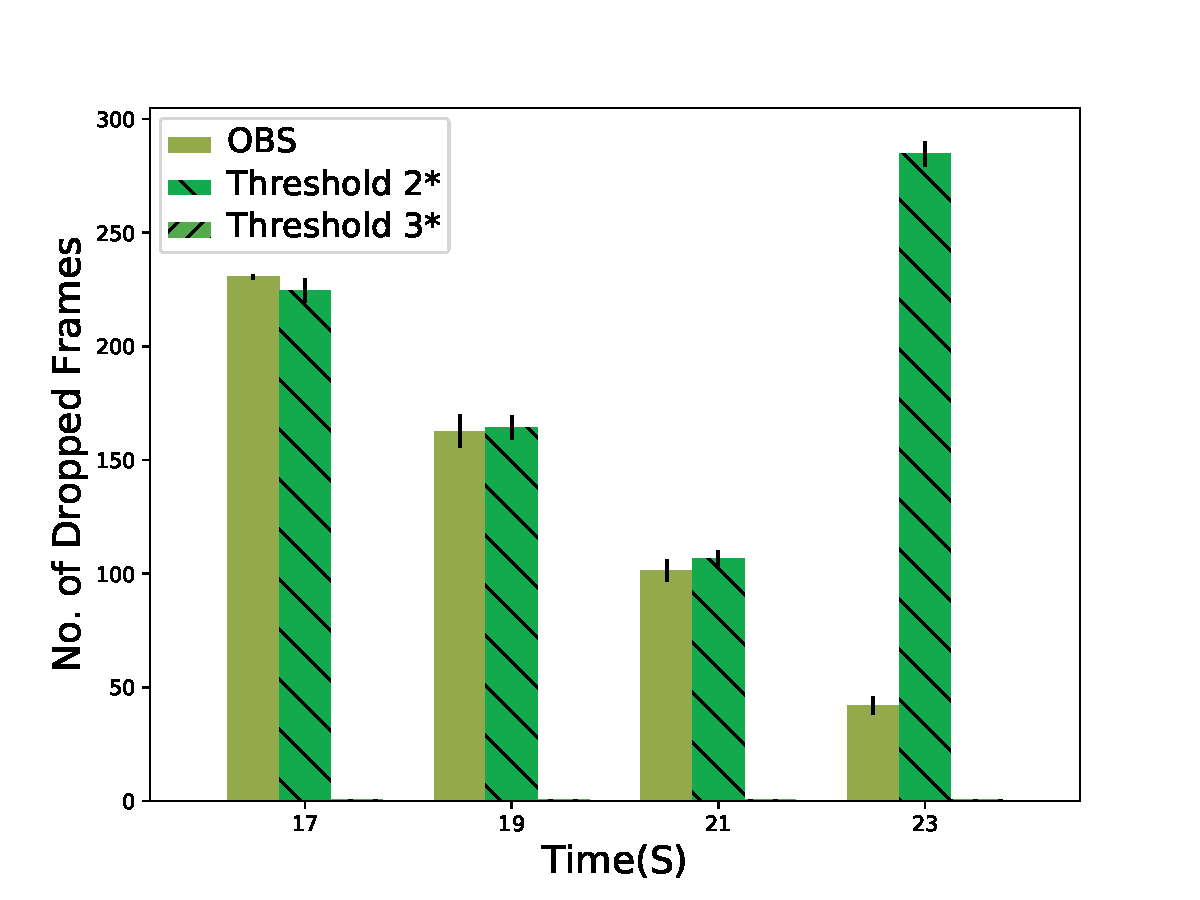
\includegraphics[width=0.32\textwidth]{fig/eval_threshold_drop.pdf}
\caption{Timeliness with varying threshold}
\label{fig:threshold-timeliness}\mylabel{fig:threshold-timeliness}
\end{figure}
\fi 
\textbf{Varying key frame interval.} OBS has a default I frame interval of 8 seconds, and we adjust it to be 4s and 2s in experiments. The frame drop are shown in Figure~\ref{fig:iframe-drop}. We can observe that in each individual experiment, when the interruption starts earlier in a GOP, more frames are dropped, because an early frame has more following frames depending on it. For example, in OBS, when interruption starts at 17s, 19s, 21s, and 23s, the number of frame drop is xx, xx, xx, and xx.
Also, the number of frame drop appears to have the same period with the keyframe interval (e.g., when keyframe interval is 4s, the number of frame drop is xx, xx, xx, and xx when interruption starts at 17s, 19s, 21s, and 23s, showing a period of 4s.).

Comparing bars within the group of 17s, we find that smaller keyframe interval significantly reduces the number of frame drop (i.e., from xx, to xx, and xx when the interval is from 8s to 4s and 2s). However, this reduction is not significant for the group of 23s, because 23s is near the end of a GOP in all cases (8s, 4s, and 2s interval), there are only 1-second frames depending on the frame at 23s.

This experiment shows that if we can eliminate the dependency between frames, an occasional network jitter would only affect frames within a limited duration near the jitter, not cascadingly affecting frames in following several seconds. In practical use, reducing keyframe interval is an intractable issue because that adjust would cause video quality degradation. A tradeoff between video quality degradation and frame dropping needs to seriously solved.

\begin{table}[htb]
\centering
\caption{No. of Dropped Frames}
\label{tab:bitrate}\mylabel{tab:bitrate}

\begin{tabular}{|l|l|l|l|l|}
\hline
Bitrate(kbps)          & 1000  & 1500  & 2000  & 2500  \\ \hline
Average Dropped Frames & 148.2 & 148.2 & 149.0 & 150.6 \\ \hline
\end{tabular}
\end{table}
\textbf{Varying bitrate.}
To make the conclusion more visible, we fix key frame interval to be 8s and introduce network interruption between 19s and 21s. In different experiments, we provide sufficient network bandwidth and vary the bitrate to be 1000kbps, 1500kbps, 2000kbps, and 2500kbps. The frame drop is shown in Table~\ref{tab:bitrate}. The different bitrates do not make much difference, the number of drop in all cases is about 149.

\textbf{Summary.} We summarize and get conclusions. First, reducing keyframe interval leads to less frame drop. Second, bitrate does not influence frame drop for the short-term case, but the quality of each picture. Preliminary Evaluation points out that a small GoP is one useful try.
